%!TEX program = xelatex 
%!TEX encoding = UTF-8 unicode
\documentclass[UTF8,nofonts]{ctexart}
\setCJKmainfont[BoldFont=STHeiti,ItalicFont=STKaiti]{STSong}
\setCJKsansfont[BoldFont=STHeiti]{STXihei}
\setCJKmonofont{STFangsong}
\setmonofont{Menlo}
\setcounter{secnumdepth}{5}
\usepackage[hmarginratio=1:1]{geometry}
\usepackage{array,float,graphicx}
\usepackage{pstricks-add}
% \usepackage{minted}
\usepackage{hyperref}
\usepackage{color,subfigure}
\usepackage{amsmath}
\usepackage{ulem,diagbox}
%表格style
\newcolumntype{L}[1]{>{\vspace{0.5em}\begin{minipage}{#1}\raggedright\let\newline\\
\arraybackslash\hspace{0pt}}m{#1}<{\end{minipage}\vspace{0.5em}}}
\newcolumntype{R}[1]{>{\vspace{0.5em}\begin{minipage}{#1}\raggedleft\let\newline\\
\arraybackslash\hspace{0pt}}m{#1}<{\end{minipage}\vspace{0.5em}}}
\newcolumntype{C}[1]{>{\vspace{0.5em}\begin{minipage}{#1}\centering\let\newline\\
\arraybackslash\hspace{0pt}}m{#1}<{\end{minipage}\vspace{0.5em}}}
%section style
\makeatletter
\renewcommand{\section}{\@startsection{section}{1}{0mm}
  {-\baselineskip}{0.5\baselineskip}{\fontsize{16pt}{16pt}\bf\leftline}}
\makeatother

\newcommand{\bhref}[2]{
\textcolor{blue}{\href{#1}{#2}}
}
\newcommand*\xor{\mathbin{\oplus}}
\newcommand*\mylshift{<\kern -.3em <}
\definecolor{bg}{rgb}{0.95,0.95,0.95}
\makeatother
%引用style
\makeatletter
\def\@cite#1#2{\textsuperscript{[{#1\if@tempswa , #2\fi}]}}
\makeatother
\pagestyle{empty}
\usepackage{fancyhdr}
%代码style
\usepackage{listings}
\usepackage{xcolor}

%封面
\title{
\fontsize{26pt}{26pt}
天气应用需求与设计分析报告
%垂直间距
\vskip 20em
}
\author{
软件工程1102班 \ \ \ 靳杰 \ \ \ U201112375
}
\date{}
\thispagestyle{empty}

\begin{document}
% 设置代码的显示
\lstset{
numbers=left,
% numberstyle=\tiny,
basicstyle=\footnotesize\ttfamily,
keywordstyle=\color{blue!90}\bfseries, % 代码关键字为蓝色,粗体
commentstyle=\color{red!50!green!50!blue!50},
frame=shadowbox,  % 把代码用带有阴影的框圈起来
rulesepcolor=\color{red!20!green!20!blue!20},
breaklines=true,  % 对过长的代码自动换行
tabsize=4, 		  % tab的大小
showstringspaces=false, % 显示字符串中的空格
keepspaces=true,
showspaces=false
}

\maketitle

\thispagestyle{empty}
\newpage
%目录
\tableofcontents
\newpage
\thispagestyle{fancy} % IEEE模板在\maketitle后会自动声明\thispagestyle{plain},
\lhead{} % 页眉左,需要东西的话就在{}内添加
\chead{} % 页眉中
\rhead{} % 页眉右
\lfoot{} % 页眉左
\cfoot{} % 页眉中
\rfoot{\thepage} %页眉右,\thepage 表示当前页码
\renewcommand{\headrulewidth}{0pt} %改为0pt即可去掉页眉下面的横线
\renewcommand{\footrulewidth}{0pt} %改为0pt即可去掉页脚上面的横线
\pagestyle{fancy}
\setcounter{page}{1}

\section{天气应用需求分析}
\subsection{需求描述}
基于iOS手机操作系统,制作一款天气应用,实现以下基本功能点:

\begin{itemize}
 	\item 从中国天气网,webservice获取指定的城市天气信息,并可在系统中显示当前天气情况。
 	\item 用sqlite数据库保存获取的历史天气信息,查阅存储的历史天气。
 	\item 对以往的天气情况进行统计,各类天气的数量,百分比。
 	\item 绘制温度的变化曲线图。
\end{itemize} 

\subsection{需求分析}
\subsubsection{应用范围} % (fold)
\label{ssub:应用范围}
系统运行在iOS移动操作系统平台上,要求iOS 7.0及以上。适用机型:iPhone4、iPhone4s、iPhone5、iPhone5s。

\subsubsection{应用功能点定义} % (fold)
\label{ssub:应用功能定义_}
\begin{itemize}
	\item 定位当前城市,显示当前天气情况。
	\item 更改城市,显示指定城市天气情况。
	\item 绘制温度变化曲线图。
	\item 查询存储的天气情况。
\end{itemize}

\section{系统设计} % (fold)
\label{sec:系统设计_}
\subsection{类图设计}
采用MVC模式设计,得到View层,Control层与Model层类图:
\vskip 10em

\begin{figure}[hbt]
\centering
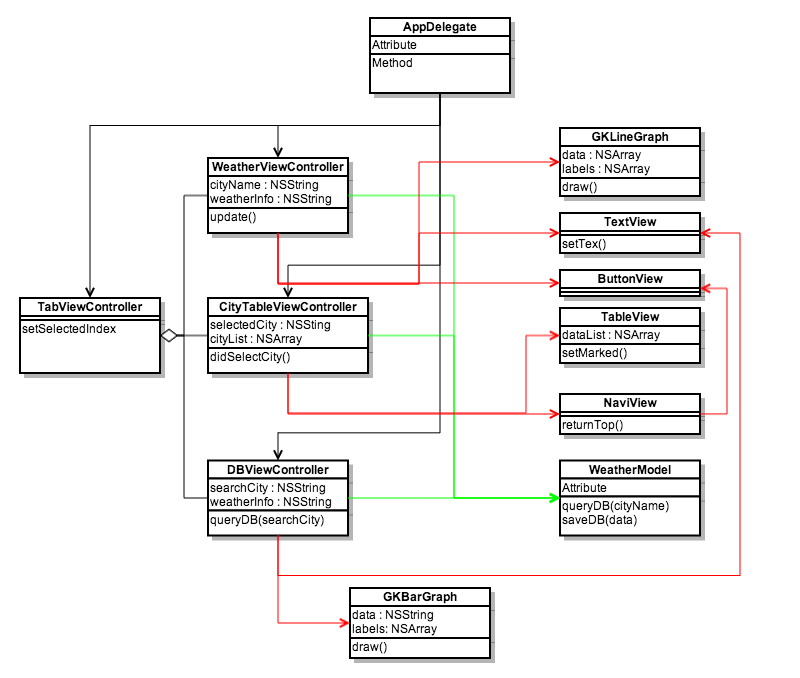
\includegraphics[width=\textwidth]{Embed.png}
\caption{系统类图}
\end{figure}

\subsection{部分算法设计} % (fold)
\subsubsection{城市定位}

未采用iOS系统自带的GPS定位信息,使用的是通过网络ip进行定位。网络地址为 \url{http://61.4.185.48:81/g/}, 通过这个网络地址可以得到一个json格式字符串,解析字符串可以得到当前网络ip对应的城市代号。

\newpage
关键代码:

\begin{lstlisting}[language={[ANSI]C++}]
//	通过ip定位当前城市 获取城市天气代码
NSURL *url = [NSURL URLWithString:@"http://61.4.185.48:81/g/"];

//	定义一个NSError对象,用于捕获错误信息
NSError *error;
NSString *jsonString = [NSString stringWithContentsOfURL:url encoding:NSUTF8StringEncoding error:&error];
//    NSLog(@"------------%@",jsonString);
if (jsonString != NULL) {
    NSString *intString;
    NSString *Str;
    for (int i = 0; i<=[jsonString length]; i++) {
        for (int j = i+1; j <= [jsonString length]; j++) {
            Str = [jsonString substringWithRange:NSMakeRange(i, j-i)];
            if ([Str isEqualToString:@"id"]) {
                if (![[jsonString substringWithRange:NSMakeRange(i+3, 1)] isEqualToString:@"c"]) {
                    intString = [jsonString substringWithRange:NSMakeRange(i+3, 9)];
                }
            }
        }
    }
    self.wM = [WeatherModel getInstance];
    [self.wM startWithNum:intString];
    [self.message setText:@"定位成功!"];
    // 设置cityTableViewController 的城市名为当前城市
}
\end{lstlisting}

\subsubsection{获取天气信息}
使用中国天气网api: http://m.weather.com.cn/atad/城市代号.html 。国内每一个城市都对应有一个城市代号,通过访问相应的网络地址,可以获得json格式数据,解析数据得到城市天气信息。

关键代码:

\begin{lstlisting}[language={[ANSI]C++}]
// 通过城市编号开始获取数据
- (void)startWithNum:(NSString *)thecityNum{
    //向开源的地址发送连接请求
    //这里使用的是异步的请求
    NSString *urlString = [NSString stringWithFormat:@"http://m.weather.com.cn/data/%@.html", thecityNum];
    NSURL *url = [NSURL URLWithString:urlString];
    NSURLRequest    *urlRequest = [NSURLRequest requestWithURL:url cachePolicy:NSURLRequestReturnCacheDataElseLoad timeoutInterval:30];
    NSURLConnection *urlConnection = [NSURLConnection connectionWithRequest:urlRequest delegate:self];
    [urlConnection start];
}

#pragma mark - NSURLConnectionDataDelegate methods
// 获取数据失败后显示网络连接失败
- (void)connection:(NSURLConnection *)connection didFailWithError:(NSError *)error{
    UIAlertView * alertV = [[UIAlertView alloc] initWithTitle:@"网络连接失败" message:[NSString  stringWithFormat:@"%@",error] delegate:self cancelButtonTitle:nil otherButtonTitles:nil, nil];
    [alertV show];
}
// 获取数据后存入数据库
- (void)connection:(NSURLConnection *)connection didReceiveData:(NSData *)data{
    // 网络返回的 JSON 数据 data
    self.m_JsonData = data;
    NSError *error = nil;
    NSDictionary *dict  = [NSJSONSerialization JSONObjectWithData:self.m_JsonData options:NSJSONReadingMutableLeaves error:&error];
    id weatherInfo = [dict objectForKey:@"weatherinfo"];
    
    self.cityName = [weatherInfo objectForKey:@"city"];
	//  解决拿到空数据的情况
    if ( self.cityName == nil) {
        //	显示警告
        [[FirstViewController getInstance] showWarring];
        return;
    }
	//	存储数据
	//	略    
}
\end{lstlisting}

\subsubsection{数据存储与查询} % (fold)
采用sqlite数据库,在iOS应用开发中,需要导入 libsqlite3.dylib 动态库。

数据存储与更新关键代码:
\begin{lstlisting}[language={[ANSI]C++}]
// 数据储存与更新
- (void) sqliteOpen{
    sqlite3 *database;
    if (sqlite3_open([[self dataFilePath] UTF8String], &database) != SQLITE_OK) {
	    // 数据库创建失败!
        sqlite3_close(database);
        NSAssert(0, @"open database faid!");
    }
    else{
        // 创建数据库语句
        NSString *ceateSQL = @"CREATE TABLE IF NOT EXISTS weather(cityName TEXT primary key,cityNum TEXT,cityInfo TEXT, date TEXT, week TEXT, temp1 TEXT, temp2 TEXT, temp3 TEXT, temp4 TEXT, temp5 TEXT, temp6 TEXT, weather1 TEXT, weather2 TEXT, weather3 TEXT, weather4 TEXT, weather5 TEXT, weather6 TEXT, img1 TEXT, img2 TEXT, img3 TEXT, img4 TEXT, img5 TEXT, img6 TEXT)";
        
        char *ERROR;
        if (sqlite3_exec(database, [ceateSQL UTF8String], NULL, NULL, &ERROR) != SQLITE_OK){
            sqlite3_close(database);
            // 表创建失败
            NSAssert(0, @"ceate table faild!");
        }
        else {
            char *saveSQL = "INSERT OR REPLACE INTO weather(cityName ,cityNum ,cityInfo , date , week , temp1 , temp2 , temp3 , temp4 , temp5 , temp6 , weather1 , weather2 , weather3 , weather4 , weather5 , weather6 , img1, img2, img3, img4, img5, img6)""VALUES(?,?,?,?,?,?,?,?,?,?,?,?,?,?,?,?,?,?,?,?,?,?,?);";
            char *errorMsg = NULL;
            sqlite3_stmt *stmt;
            if (sqlite3_prepare_v2(database, saveSQL, -1, &stmt, nil) == SQLITE_OK) {
                
                sqlite3_bind_text(stmt, 1, [self.cityName UTF8String], -1, NULL);
                ... // 略
            }
            // 数据更新失败
            if (sqlite3_step(stmt) != SQLITE_DONE) {
                NSAssert(0, @"error updating :%s",errorMsg);
            }
            sqlite3_finalize(stmt);
            sqlite3_close(database);
        }
    }
}
\end{lstlisting}
数据查询关键代码:
\begin{lstlisting}[language={C++}]
// 获取app内文件路径函数
-(NSString *) dataFilePath{
    NSArray *path =  NSSearchPathForDirectoriesInDomains(NSDocumentDirectory, NSUserDomainMask, YES);
    NSString *document = [path objectAtIndex:0];
    return [document stringByAppendingPathComponent:@"weather.sqlite"];
}
// 查找数据库
-(BOOL) sqliteCheck{
    sqlite3 *database;
    BOOL returnValue = YES;
    // 数据库查找失败!
    if (sqlite3_open([[self dataFilePath] UTF8String], &database) != SQLITE_OK) {
        sqlite3_close(database);
        NSAssert(0, @"open database failed!");
        return false;
    }
    else{
    	// 查询语句
        NSString *query= [NSString stringWithFormat:@"select * from weather where cityName = '%@'", [CityTableViewController getCurrentCity]];
        sqlite3_stmt *stmt;
        if (sqlite3_prepare_v2(database, [query UTF8String], -1, &stmt, nil) == SQLITE_OK) {
            returnValue = false;
            while (sqlite3_step(stmt) == SQLITE_ROW) {
                self.cityName = [[NSString alloc] initWithUTF8String:(char*)sqlite3_column_text(stmt, 1-1)];
                ... // 略
                returnValue = true;
            }
        }
        else{
        	// 查询失败
            NSLog(@"%s",sqlite3_errmsg(database));
            returnValue = false;
        }
        sqlite3_finalize(stmt);
    }
    //用完了一定记得关闭,释放内存
    sqlite3_close(database);
    return returnValue;
}
\end{lstlisting}

\section{总结} 
\label{sec:总结_}
项目网络托管地址 \url{https://github.com/jinjaysnow/Snow} 。

此次实验大作业编写iOS平台的天气应用程序,是我自己第一次较全面(网络编程、数据库、UI、多视图控制)的制作iOS平台应用程序。万事开头难,通过这次实验,了解了iOS应用程序开发的基本流程和应用程序整个生命周期的运作方式,获得了基本的 \textit{\textbf{Objective-C}}编程技巧。收获较大。

\section{系统截图展示} 
\label{sec:系统截图展示_}
\begin{figure}[hbt]
\centering

\includegraphics[width=0.8\textwidth]{1.png}
\caption{系统欢迎界面}
\end{figure}
\begin{figure}[hbt]
\centering

\includegraphics[width=0.8\textwidth]{2.png}
\caption{系统启动界面}
\end{figure}
\begin{figure}[hbt]
\centering
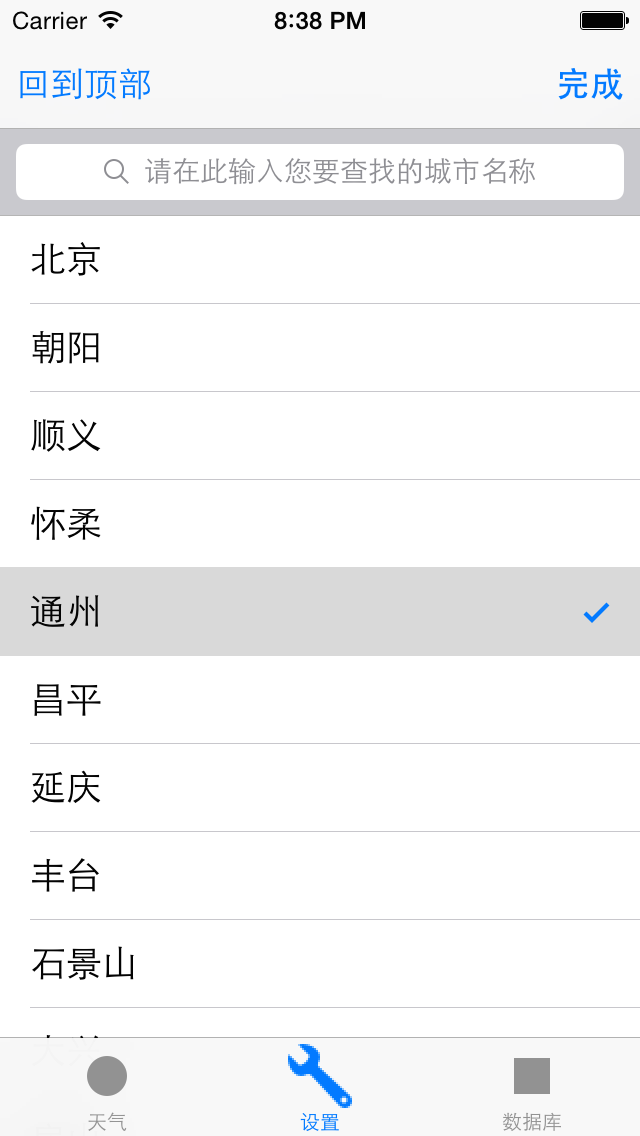
\includegraphics[width=0.8\textwidth]{3.png}
\caption{城市选择界面}
\end{figure}
\begin{figure}[hbt]
\centering
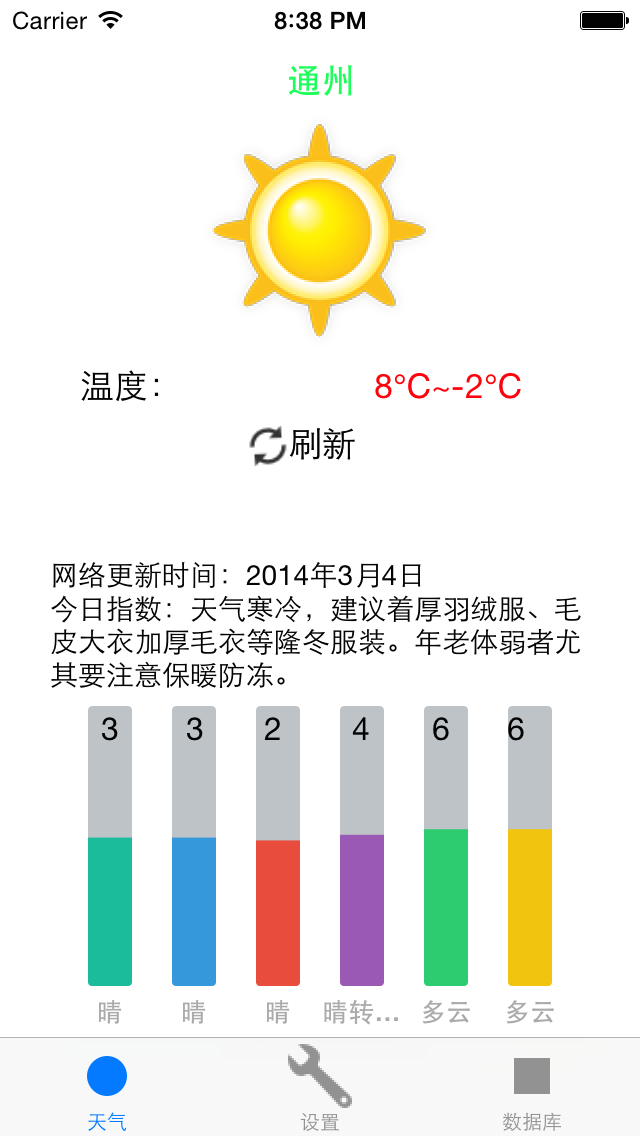
\includegraphics[width=0.8\textwidth]{4.png}
\caption{选择城市后更新界面}
\end{figure}
\begin{figure}[hbt]
\centering

\includegraphics[width=0.8\textwidth]{5.png}
\caption{城市搜索界面}
\end{figure}
\begin{figure}[hbt]
\centering
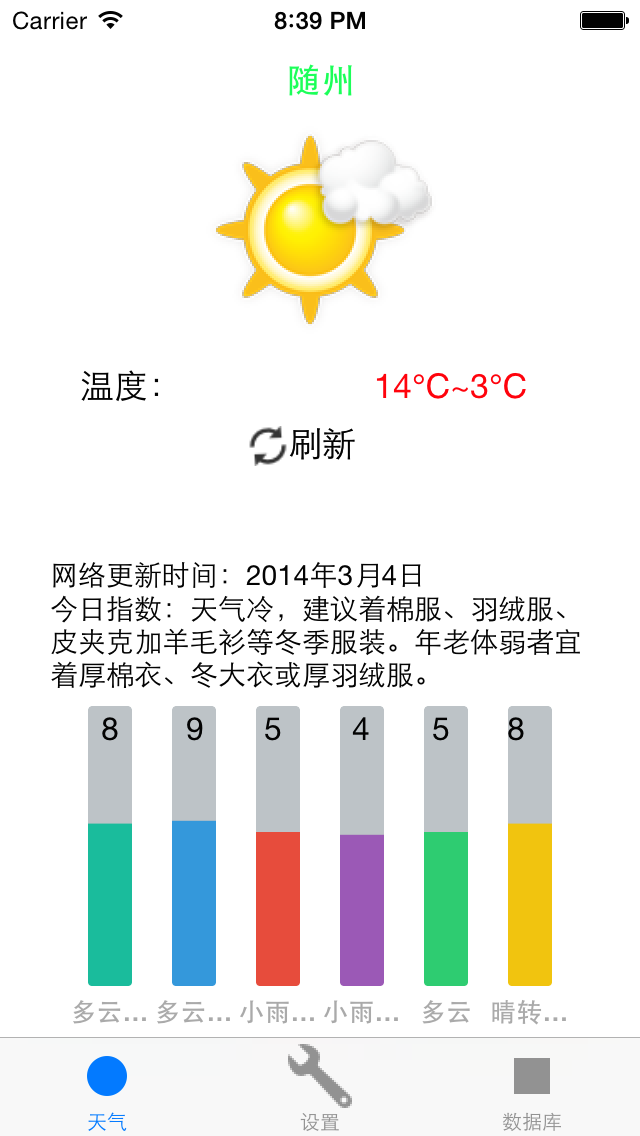
\includegraphics[width=0.8\textwidth]{6.png}
\caption{搜索后更新界面}
\end{figure}
\begin{figure}[hbt]
\centering
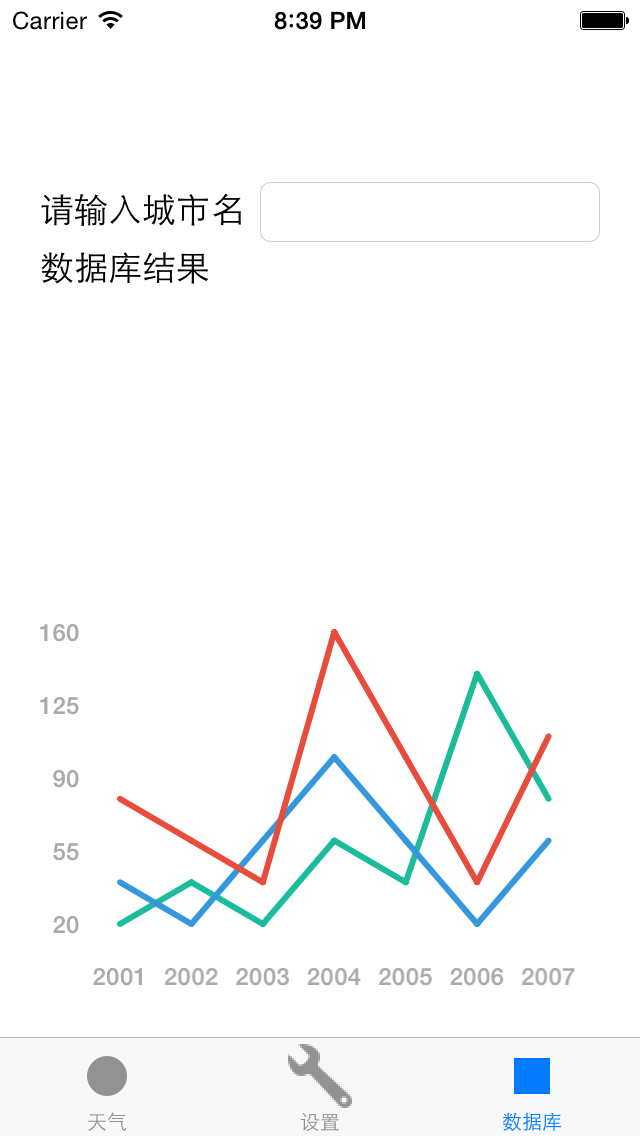
\includegraphics[width=0.8\textwidth]{7.png}
\caption{数据库界面}
\end{figure}
\begin{figure}[hbt]
\centering

\includegraphics[width=0.8\textwidth]{8.png}
\caption{数据库搜索界面}
\end{figure}
\begin{figure}[hbt]
\centering

\includegraphics[width=0.8\textwidth]{9.png}
\caption{数据库搜索结果展示}
\end{figure}
% section 系统截图展示_ (end)
\end{document}